\documentclass{article}
\usepackage{amsmath}
\usepackage[margin=1in]{geometry}
\usepackage{marginnote}
\usepackage{gensymb}
\usepackage{enumitem}
\usepackage{graphicx}
\usepackage{float}
\usepackage[numbers]{natbib}
\usepackage{xcolor}

\newcommand{\cosec}{\, \mathrm{cosec}}
\graphicspath{ {./Images/} }

\begin{document}

\title{\textbf{HPES PDF Scanner \\ IEDP - Image Median Filtering \& Edge Detection}}
\author{\textcolor{gray!150}{Project Team:} \\
\textcolor{gray!150}{Caide Lander – LNDCAI001 $\rightarrow$ Research and machine learning specialist}\\
\textcolor{gray!150}{Lloyd Ross – RSSLLO001 $\rightarrow$ FPGA and Protyping specialist} \\
\textcolor{gray!150}{Francis Mutetwa – MTTFRA005 $\rightarrow$ Golden Measure and algorithm specialist}\\
\textcolor{gray!150}{Dante Webber – WBBDAN003 $\rightarrow$ Team Leader and algorithm specialist}}
\date{\today}

\maketitle

\begin{abstract}
    An independent embedded system that can take an image of a desired page, and after implementing the appropriate pre-processing 
    such as noise reduction through median filtering and edge detection of the page and text for accurate, can convert the image to 
    a PDF file and output it to a connected computer.
\end{abstract}

\begin{figure}[H]
    \centering
    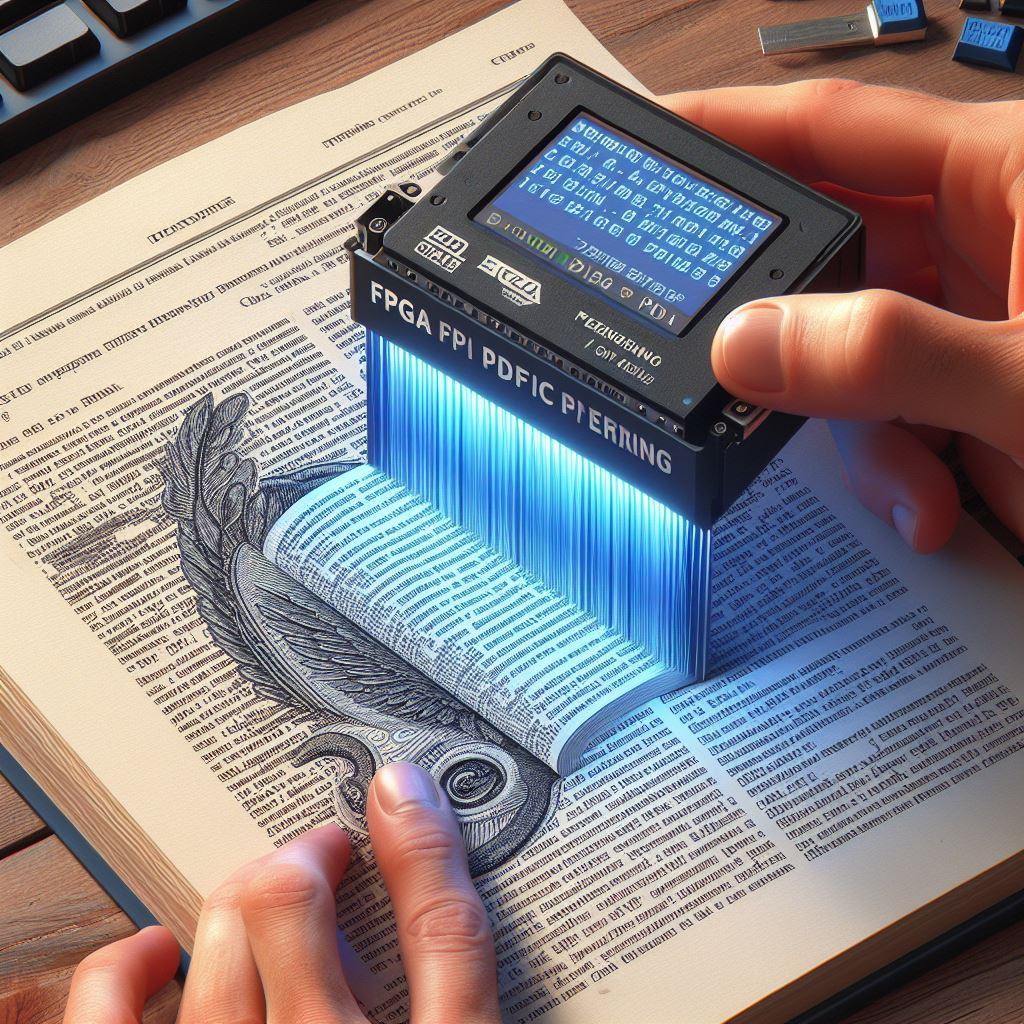
\includegraphics[width=0.7\textwidth]{Images/OIG1.jpeg}
    \caption{A Microsoft copilot interpretation of an FPGA PDF Scanner}
    \label{fig:Figure 1}
\end{figure}

\section*{Project Description}
The aim of this project is to create an independent document-image processor using median filtering and edge detection. 

At base level the device will be able to take in an image input - formatted in arrays of the pixel colour values by 
\texttt{width x height} (.bmp). The device will then process the image through appropriate algorithms including median filtering and edge 
detection, and finally convert the image to a PDF file.

\subsection*{Median Filtering}
Median filtering is an image processing algorithm that calculates and re-populates pixel values in an image based on the 
median value of the surrounding pixels. This process helps to remove noise from images while preserving the edges of objects 
in the images. This is important for ‘pdf’ scanning because each printed item (word, letter, etc.) on a page is an object that 
will need to be detected later, so edges need to be preserved, and noisy images will make it harder to detect the valuable information 
(the objects). A flow chart detailing the concept behind the algorithm is shown below. 

\begin{figure}[H]
    \centering
    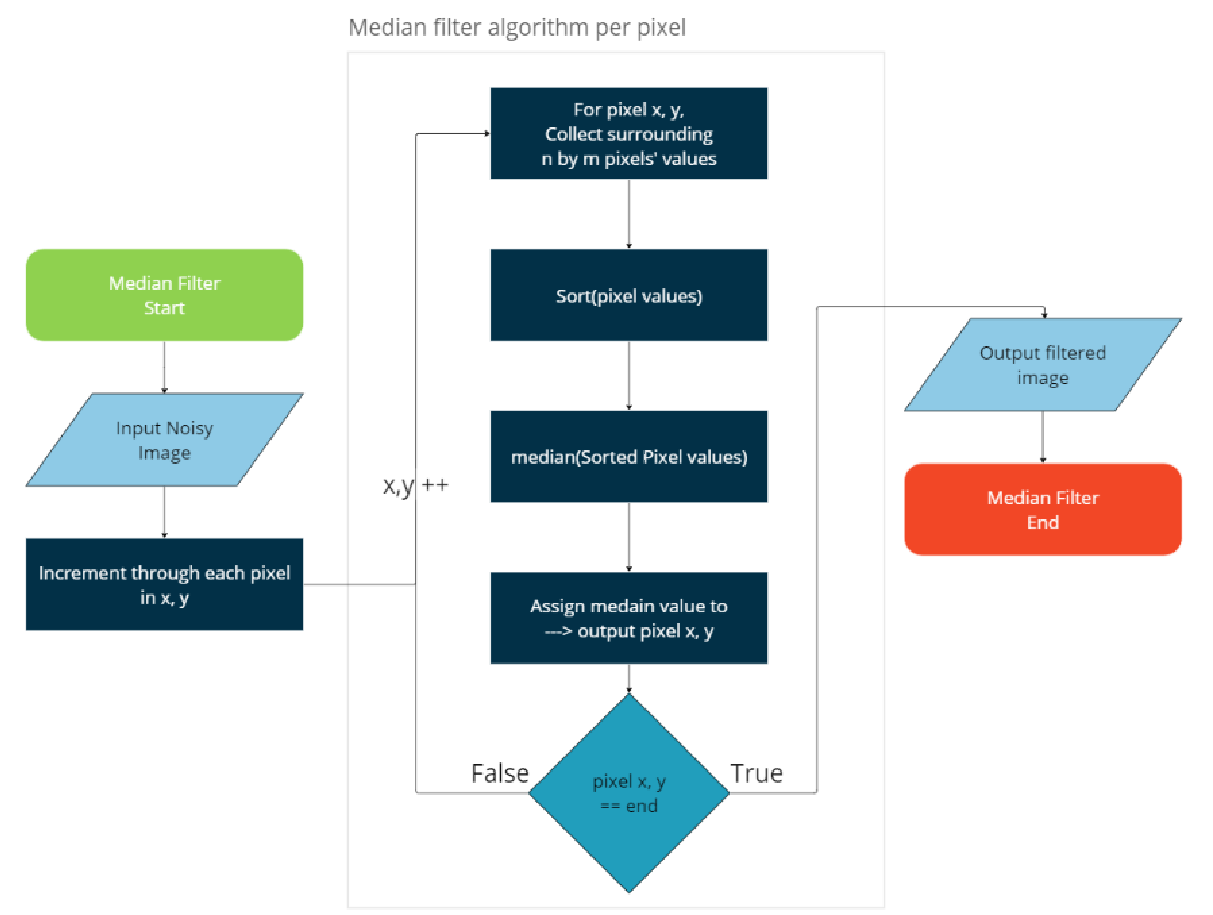
\includegraphics[width=0.5\textwidth]{Images/Median_Filter_Block_Diagram.png}
    \caption{Median Filter Flow Chart}
    \label{fig:Figure 2}
\end{figure}

\subsection*{Edge Detection and Processing}

Edges in images represent areas with significant changes in intensity or colours, marking transitions between different objects or 
regions within the image. Detecting these edges is crucial for computer vision and various image processing tasks, including document-image 
processing for accurate PDF generation \cite{nagalakshmi2015}. \medskip

When aiming to accelerate edge detection on an FPGA, it is necessary to prioritize algorithms that align well with the FPGA's hardware 
architecture. Given this requirement - the Sobel and Prewitt operators are favourable choices due to their simplicity and efficient 
parallelization potential on FPGA hardware \cite{6949951}. Additionally, the Roberts Cross operator, with its straightforward computation, is 
suitable for FPGA implementation, particularly in resource-constrained environments. \medskip

Sobel and Prewitt Operators: These operators perform convolution with simple 3x3 kernels to compute the gradient magnitude and direction. 
Its straightforward computation makes it well-suited for FPGA implementation, where parallelism can be utilised to compute gradients for 
multiple pixels simultaneously \cite{6949951}. \medskip

Canny Edge Detector: While the Canny edge detector offers high-quality edge detection, its multi-stage algorithm and non-linear operations 
may pose challenges for FPGA implementation. However, with careful optimizations and efficient resource utilization, including optimizations 
for the non-maximum suppression and hysteresis thresholding stages, the Canny detector can still be effectively implemented on an FPGA \cite{6774938}. \medskip

In addition to traditional edge-detection algorithms, the project aims to explore the potential of machine learning for edge detection. 
Machine learning has been used in various image processing tasks, including edge detection, by learning from large datasets to identify 
complex patterns and features within images. Integrating this into the image scanner and processor can enhance the system's ability to 
detect edges accurately, especially in scenarios with varying edge complexities and noise levels. 

\subsection*{Connected Components}
A connected component is an image processing term that refers to neighbouring pixels that all have an intensity value (for grayscale images) 
or colour (for coloured images) that falls within/above a custom defined threshold. This algorithm/tool can be used to find groups of 
connected pixels on a page, such as a letter (should consist of darker pixels than the page-colour pixels surrounding it). This will aid in text 
recognition algorithms, as the text can be isolated and then compared.

\section*{Prototype Specification}
\begin{itemize}
    \item The system will be initially simulated in Verilog to confirm the concepts functionality. 
    \item The prototyping will then be done on an FPGA using the Nexys4 \cite{digilentN4}. 
    \item Image to be processed must be converted into or stored in bitmap format (.bmp). 
    \item There will be support for USB input and output communication. 
    \item The device will be able to idle while waiting for a trigger (input).  
    \item The device will be triggered when there is an image input sent to it.
    \item The device will be able to convert the image to a PDF file type.
    \item The device will be able to send the processed PDF file through the USB communication infrastructure.
\end{itemize}

\begin{figure}[H]
    \centering
    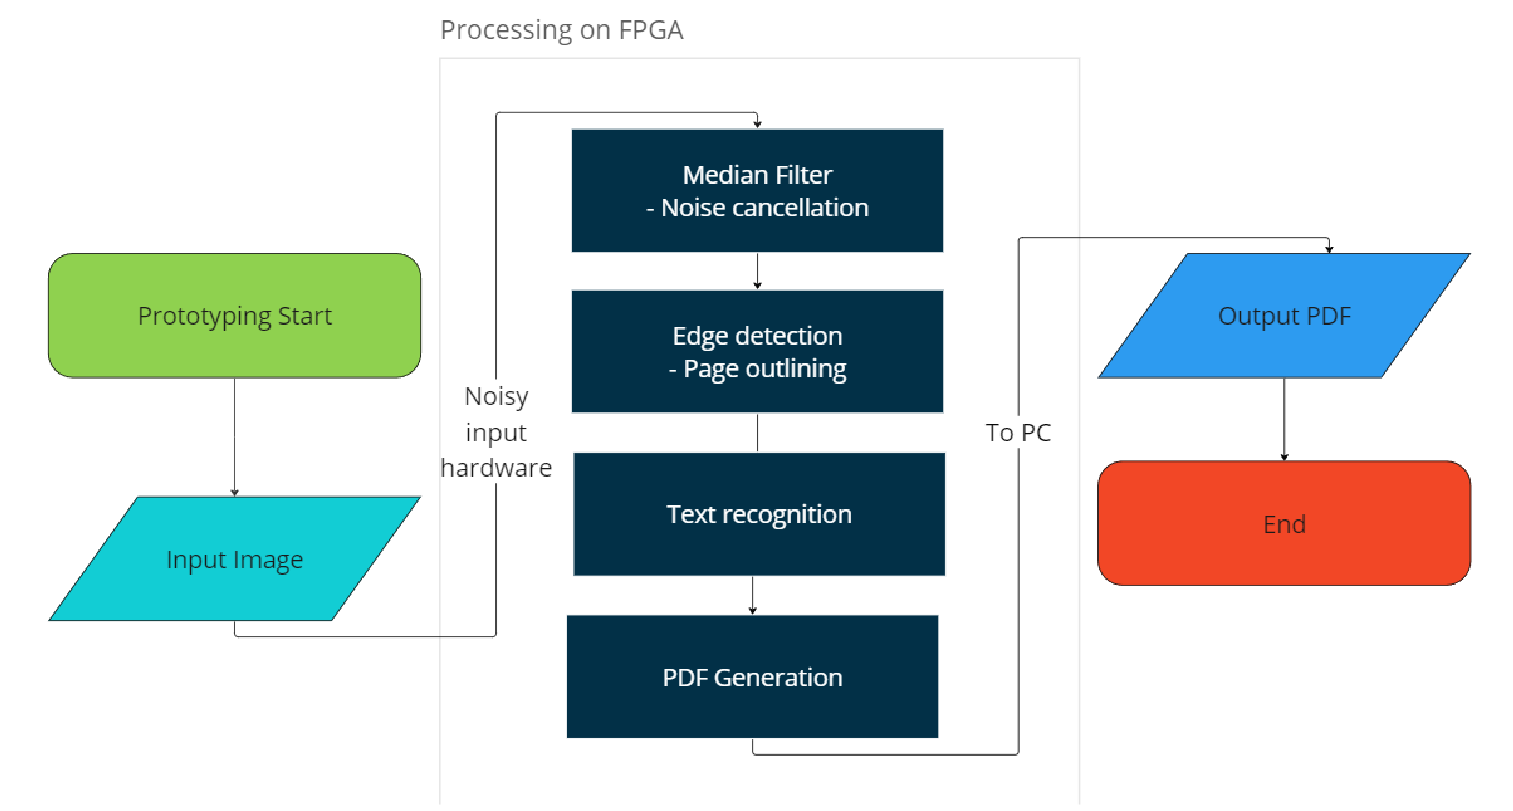
\includegraphics[width=0.5\textwidth]{Images/Prototype_Concept_Flow_Chart.png}
    \caption{Base level prototype concept flow chart}
    \label{fig:Figure 3}
\end{figure}

\section*{Project Goals}
\begin{itemize}
    \item Starts up. 
    \item Can interpret a bitmap image input. 
    \item Can detect noise. 
    \item Can filter irregularities due to noise using median filter. 
    \item Can determine edges of page from image. 
    \item Can recognize text. 
    \item Can generate a pdf of page image. 
    \item Can successfully output PDF to computer. 
    \item Accelerate processes using parallelization. 
\end{itemize}
If physical prototyping fails, the project goals are to be achieved on a thorough testbench simulation using HDL. 

\bibliographystyle{IEEEtran}
\bibliography{references.bib}
\end{document}